% Fig. 2.20 / spec Fig A22 -- Chebyshev's inequality: the central interval
%   mu_X +- k sigma_X carries at least 1 - 1/k^2 of the probability.
% Source: mathstatch2.tex lines 3682-3726.
%
% Density.  The manuscript draws 45/4 x^3 e^{-1.7x} - 0.15 + 1.5 e^{-3(x-4)^2}
% and then marks mu_X at 2.6, which is not the expectation of that curve (and
% the curve is not a density: it does not integrate to 1 and is cut off flat at
% both ends).  Spec 3.2 item 6 and the last line of spec A22 require a bimodal
% mixture whose expectation and standard deviation can actually be computed, so
% this file draws
%     f(x) = 0.6 N(2, 0.6^2) + 0.4 N(4, 0.45^2)
%          = 0.3989423 e^{-(x-2)^2/0.72} + 0.3546154 e^{-(x-4)^2/0.405},
% the two coefficients being 0.6/(0.6 sqrt(2 pi)) and 0.4/(0.45 sqrt(2 pi)).
% Its moments are exact:
%     mu_X   = 0.6(2) + 0.4(4) = 2.8
%     E(X^2) = 0.6(0.36 + 4) + 0.4(0.2025 + 16) = 9.097
%     Var(X) = 9.097 - 7.84 = 1.257,  sigma_X = 1.1211601
% and with k = 1.3, k sigma_X = 1.4575081, so the three boundaries stand at
%     mu_X - k sigma_X = 1.3424919   f = 0.2188479 -> 1.6632cm
%     mu_X             = 2.8         f = 0.1741398 -> 1.3235cm
%     mu_X + k sigma_X = 4.2575081   f = 0.3013948 -> 2.2906cm
% and the bound is 1 - 1/k^2 = 1 - 1/1.69 = 0.4082840.  (The interval in fact
% carries 0.8045740; Chebyshev's bound is not tight, which is the point of the
% surrounding text.)  Other heights, at y = 7.6cm: f(2) = 0.3989605 -> 3.0321cm
% and f(4) = 0.3561576 -> 2.7068cm at the two component centres, f(3) =
% 0.1294982 -> 0.9842cm between them.  The true local maxima stand a little off
% the component centres, at x = 2.0001626 (0.3989605) and x = 3.9949813
% (0.3561791), and the true minimum is at x = 3.1114426 (0.1222243), not at
% x = 3; none of the six is used as a drawing input, since the curve is plotted
% from the formula, and they are recorded here only for checking.
%
% Layout.  Two faults of the manuscript picture, both listed in spec 3.2, are
% fixed here:
%   - item 12: the label inside the shading is \footnotesize there, which falls
%     under the 12px floor of spec 1.3 at the 350px phone width.  It is \small
%     here and shortened to P(.), the full event being written in the caption;
%   - item 11: the manuscript starts the callout arrow 0.1cm above that label.
%     Here the label sits at (1.95, 1.00cm), under the left mode, and the arrow
%     starts at (2.48, 1.42cm), which is 0.79cm below the curve and 0.29cm
%     inside the right edge of the shading at that height, and 0.39cm from the
%     nearest corner of the label's box.
% The arrow leaves the shading through the curve at x = 2.67, passes 0.229cm
% above the right mode and its head stops 0.236cm short of the first glyph of
% the label; it clears the tops of all three dashed boundaries, so no dashed
% line crosses another.  It is an explicit cubic Bezier rather than a bend, so
% that these clearances follow from the coordinates.
%
% The three axis labels cannot share one row: each of the outer two is 1.657cm
% wide against centres 1.4575cm apart.  Per spec 1.3 they are staggered, mu_X
% alone on the upper row and the two outer ones on the lower, where they clear
% each other by 1.32cm; the rows clear each other by 0.258cm vertically.
%
% Deviations from CH2_FIGURE_SPECS.md:
%
% 1. None of the coordinates of spec A22 are used, for the reason given above.
%    The picture keeps its arrangement -- bimodal curve, three boundaries, the
%    central block shaded, one label inside it and one callout to the upper
%    right -- and replaces every number.
%
% 2. \DeclareMathSizes{10}{10}{9}{8} raises the math script sizes from the
%    default 7pt/5pt, as in quartiles-equal-areas.tex and
%    skewness-coefficients.tex; {9}{9}{8}{7} does the same for \small, which
%    matters here because the callout carries k^2 inside a \small formula.
%
% 3. \dfrac rather than \frac in the callout, so that its numerator and
%    denominator stand at the full 9pt of \small instead of script size.
%
% 4. The multiplier of sigma_X is written k, not the a of spec A22, after the
%    author's ruling of 2026-08-08 that throughout section 2.4 a denotes the
%    positive threshold and k the multiplier of E(X) or of sigma.  The figure
%    caption and the alt text of Fig. 2.20 were already in k; only the three
%    marks in the picture were left behind.
%
% Size and type.  Native 203.368 x 126.618 pt (drawing range 7.03cm wide,
% inside the 9.0cm cap of spec 1.3; the height was 125.511 pt while the two
% outer axis marks read a sigma_X, the ascender of k having lengthened their
% boxes by 1.107 pt downwards -- the width, which alone fixes the scale on
% the page, is unchanged).  A mark of S pt shows at
% S x 0.99626 x <display width> / 203.368 px, so for a topic-figure--wide in
% body text, which .topic-figure--wide img sizes at min(100%, 620px):
%     display width      350px (390px phone)   620px (desktop)
%     10pt \normalsize   17.15px               30.37px
%      9pt \small         15.43px               27.34px
%      8pt scripts        13.72px               24.30px
% The marks at 8pt are the X of mu_X, sigma_X and f_X (scriptscript) and the
% exponent of k^2 in the callout (script inside \small); each is a component of
% a symbol rather than a label of its own, and 13.72px is above the 12px floor
% of spec 1.3.  Measured back from the SVG, the exponent has an ink height of
% 5.281 against the 5.953 of the 1 above the fraction rule, a ratio of 0.887
% against the 8/9 of 0.889, so the {9}{9}{8}{7} declaration is doing its work;
% without it the exponent would have stood at 6.5pt, i.e. 11.1px on a phone.
\documentclass[tikz,border=2pt]{standalone}
\usepackage{amsmath}
\usepackage{amssymb}
\usepackage{xcolor}
\usetikzlibrary{arrows.meta}
\newcommand{\sssig}{\scriptscriptstyle}
\DeclareMathSizes{10}{10}{9}{8}
\DeclareMathSizes{9}{9}{8}{7}

\definecolor{journalink}{HTML}{1F1C18}
\definecolor{journalmuted}{HTML}{8A7F72}
\definecolor{journalaccent}{HTML}{9C2D2D}

% 0.6 N(2, 0.6^2) + 0.4 N(4, 0.45^2)
\newcommand{\mixture}[1]{0.3989423*exp(-((#1)-2)*((#1)-2)/0.72)
                        +0.3546154*exp(-((#1)-4)*((#1)-4)/0.405)}

\begin{document}
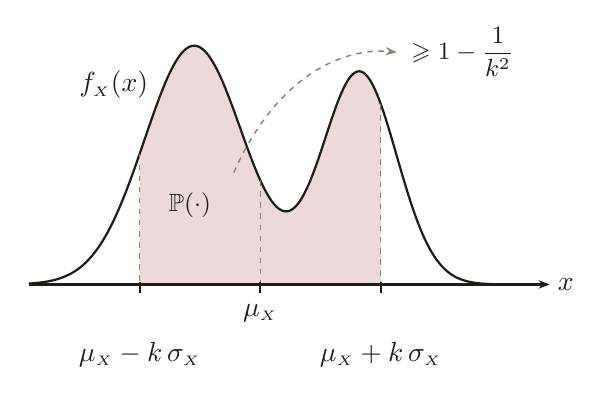
\begin{tikzpicture}[
  x=1.05cm,
  y=7.6cm,
  every node/.style={font=\normalsize, journalink},
  axis/.style={journalink, line width=0.8pt, -{Stealth[length=4pt]}},
  tick/.style={journalink, line width=0.8pt},
  curve/.style={journalink, line width=0.8pt},
  guide/.style={journalmuted, line width=0.5pt, dash pattern=on 2pt off 2pt},
  pointer/.style={journalmuted, line width=0.5pt,
                  dash pattern=on 2pt off 2pt, -{Stealth[length=4pt]}},
  central/.style={journalaccent, fill opacity=0.18}
]
  % ---- the central interval [mu - k sigma, mu + k sigma] ----------------
  % Shading path per spec 1.6: from the foot of the left boundary along the
  % x axis to the foot of the right boundary, up to the curve, back along the
  % curve, cycle.
  \fill[central]
    (1.3424919,0) -- (4.2575081,0) -- (4.2575081,0.3013948)
    -- plot[domain=4.2575081:1.3424919, samples=300, smooth]
       (\x,{\mixture{\x}})
    -- cycle;

  % ---- density curve ----------------------------------------------------
  \draw[curve] plot[domain=0:6, samples=400, smooth] (\x,{\mixture{\x}});

  % ---- x axis -----------------------------------------------------------
  \draw[axis] (0,0) -- (6.3,0);
  \node[anchor=west, inner sep=2.8pt] at (6.3,0) {$x$};

  % ---- the three boundaries ---------------------------------------------
  \draw[guide] (1.3424919,0.2188479) -- (1.3424919,0);
  \draw[guide] (2.8,0.1741398) -- (2.8,0);
  \draw[guide] (4.2575081,0.3013948) -- (4.2575081,0);
  \foreach \p in {1.3424919, 2.8, 4.2575081}
    \draw[tick] ([yshift=0.035cm]\p,0) -- ([yshift=-0.106cm]\p,0);
  % upper row
  \node[anchor=north, inner sep=0pt] at ([yshift=-0.25cm]2.8,0)
    {$\mu_{\sssig X}$};
  % lower row
  \node[anchor=north, inner sep=0pt] at ([yshift=-0.73cm]1.3424919,0)
    {$\mu_{\sssig X}-k\,\sigma_{\sssig X}$};
  \node[anchor=north, inner sep=0pt] at ([yshift=-0.73cm]4.2575081,0)
    {$\mu_{\sssig X}+k\,\sigma_{\sssig X}$};

  % ---- curve label -------------------------------------------------------
  % Bottom right corner (1.45, 2.35cm); the curve stands 1.992cm there, so the
  % box clears it by 0.358cm, and it stands 0.687cm above the top of the left
  % boundary.
  \node[anchor=south east, inner sep=0pt] at ([yshift=2.35cm]1.45,0)
    {$f_{\sssig X}(x)$};

  % ---- the probability of the shaded interval ---------------------------
  % Inside the shading, under the left mode: the box is 0.537cm wide and
  % 0.316cm tall, so it clears the left boundary by 0.370cm, the boundary at
  % mu_X by 0.624cm and the curve above it by more than 1.7cm.
  \node[inner sep=0pt] at ([yshift=1.00cm]1.95,0)
    {\small $\mathbb{P}(\cdot)$};

  % ---- callout to the bound ---------------------------------------------
  \draw[pointer] ([yshift=1.42cm]2.48,0)
    .. controls ([yshift=2.55cm]2.95,0) and ([yshift=3.02cm]3.72,0)
    .. ([yshift=2.95cm]4.45,0);
  \node[anchor=west, inner sep=0pt] at ([yshift=2.95cm]4.62,0)
    {\small $\geqslant1-\dfrac{1}{k^{2}}$};
\end{tikzpicture}
\end{document}
